% =====================================================================
%  Score-vs-Rank Comparison Experiment — Full Experiment Report
%  Compile with:  pdflatex score_vs_rank_report.tex  (run twice)
%  Figure paths are relative to this file (outputs/...), so compile
%  from the 09_monot5_score_vs_rank/ directory.
% =====================================================================
\documentclass[11pt]{article}

\usepackage[margin=1in]{geometry}
\usepackage{amsmath, amssymb}
\usepackage{graphicx}
\usepackage{booktabs}
\usepackage{longtable}
\usepackage{array}
\usepackage{float}
\usepackage{xcolor}
\usepackage{caption}
\usepackage{enumitem}
\usepackage{listings}
\usepackage[hidelinks]{hyperref}

\definecolor{codegray}{gray}{0.95}
\lstset{
  basicstyle=\ttfamily\footnotesize,
  backgroundcolor=\color{codegray},
  breaklines=true,
  frame=single,
  columns=fullflexible,
  keepspaces=true,
}

\newcommand{\score}{\operatorname{score}}
\newcommand{\rank}{\operatorname{rank}}

\title{\textbf{Score Change vs.\ Rank Change} \\[2pt]
\large Validating monoT5's Logit-Confidence Metric Against
Parry et al.'s Rank-Based Attack Evaluation}
\author{Information-Retrieval Adversarial-Evaluation Project --- Experiment 9}
\date{\today}

\begin{document}
\maketitle

\begin{abstract}
Every other experiment in this project (Experiments~1--3, 6, 7) reports
attack strength as a \textbf{score change}:
$\Delta_{\score} = \score_{\text{attack}} - \score_{\text{control}}$, the
change in monoT5's $\operatorname{logit}(\texttt{true}){-}\operatorname{logit}(\texttt{false})$
confidence. Parry et al.'s ECIR-24 evaluation instead reports attacks as
\textbf{rank changes}: did an attacked document move up in its query's
candidate list? These are different quantities that need not agree on
every example --- a large confidence jump on a document that remains deep
in its ranking is a real, separate phenomenon from a small confidence jump
that happens to cross a rank boundary. This experiment computes both
metrics, point-wise, on the exact same curated 105-attack grid used
throughout this project (up to 500 examples per attack, no filtering, to
avoid survivorship bias), and asks whether they correlate. Across
\textbf{52{,}478 pooled examples} the two metrics correlate at
\textbf{Spearman $\rho = 0.764$}, and the per-attack scatter of mean score
change vs.\ mean rank change is visually almost linear
(Figure~\ref{fig:scatter}): every attack that raises the average score also
raises the average rank, and vice versa, with only 4 of 105 attack
configurations landing in a disagreeing quadrant, and \emph{zero} landing
in the quadrant where score improves but rank does not. This project's
score-based conclusions and Parry et al.'s rank-based conclusions are
therefore measuring genuinely correlated, mutually consistent phenomena.
Two research findings not stated in the original task shaped the design:
Experiment~8/DecoderLens's own precomputed outputs turned out to be missing
29 of the 105 curated attacks (every \texttt{relevant\_*}/\texttt{true\_*}
attack, including the project's canonical \texttt{relevant\_start\_5}), so
only its \emph{code} was reused, not its run outputs; and all 105 curated
attacks share one identical 42-query set with byte-identical BM25 top-100
candidate membership per query, making the ranking machinery's one
model-touching step a one-time, $\sim$4{,}300-example computation rather
than a per-attack one.
\end{abstract}

\tableofcontents
\newpage

% =====================================================================
\section{Introduction and Motivation}
% =====================================================================

A keyword-stuffing attack on a neural re-ranker can be measured in (at
least) two ways: by how much it changes the model's raw relevance
\emph{confidence} for the attacked document, or by how much it changes that
document's \emph{position} in a ranked list of competing candidates. This
project has so far exclusively used the first framing (Experiments~1--3, 6,
7); Parry et al.'s original ECIR-24 adversarial-evaluation paper uses the
second. Neither framing is wrong, but they are not the same measurement:

\begin{quote}
\itshape Does a change in monoT5's raw score reliably predict a change in
where the document actually ranks against its competitors --- and if the
two sometimes disagree, how often, and in which direction?
\end{quote}

This experiment answers that question directly and compactly: for every
example in every one of the 105 curated attacks, compute both
$\Delta_{\score}$ and a point-wise rank change $\Delta_{\rank}$ against a
fixed BM25 top-100 candidate set, and report how strongly the two
correlate. The purpose is explicitly \emph{validating}, not
\emph{replacing}, this project's score-based results: the goal is to show
they do not contradict Parry et al.'s protocol, while being honest about
the (small) fraction of cases where the two measures disagree in direction.

% =====================================================================
\section{Background and Reuse}
% =====================================================================

This experiment introduces almost no new methodology --- it is a
compact wiring-together of two already-verified components:

\begin{itemize}[nosep]
  \item \textbf{Experiment~1} supplies the model, the scoring function
        $\score=\operatorname{logit}(\texttt{true})-\operatorname{logit}(\texttt{false})$,
        the curated 105-attack grid (7 tokens $\times$ 3 positions $\times$
        5 repetitions --- \emph{not} Experiment~8's broader 16-token/226-attack
        superset), and, critically, the already-computed
        \texttt{outputs/attacks/\{attack\}/scores/all\_scores.csv} score
        pool (control/attack scores for up to 500 pairs per attack) ---
        meaning \textbf{target scores required zero new forward passes}.
  \item \textbf{``Experiment~8'' / DecoderLens}
        (\texttt{monot5\_decoderlens\_rank/}, unnumbered on disk but
        referred to as Experiment~8 in this project's terminology) supplies
        the fixed BM25 top-100 candidate-set construction
        (\texttt{load\_attack\_tsv}, \texttt{build\_candidate\_sets}) and
        the point-wise rank computation (\texttt{compute\_rank}): every
        candidate except the target keeps its clean score; only the
        target's score is swapped for the variant under test.
\end{itemize}

\subsection{A coverage gap that shaped the design}
\label{sec:coverage}

DecoderLens's own precomputed run (\texttt{outputs/attacks/}) was checked
against the curated 105-attack list before deciding how to reuse it. It
covers 226 attacks drawn from a 16-token superset, but \textbf{29 of the
curated 105 are absent from its successful outputs} --- every single
\texttt{relevant\_*} and \texttt{true\_*} attack, including
\texttt{relevant\_start\_5}, the one canonical attack used as a reference
point throughout Experiments~1--3. Its target cap
(\texttt{max\_target\_examples\_per\_attack: 100}) also directly conflicts
with this task's explicit ``no filtering, up to 500 examples'' requirement.
\textbf{Consequently, this experiment reuses DecoderLens's \emph{code}, not
its precomputed \emph{run outputs}}: target scores come from Experiment~1's
own \texttt{all\_scores.csv} (zero forward passes), and only the $\sim$100
candidates per query needed fresh clean scoring.

\subsection{A shared-query discovery that made the candidate scoring cheap}

Before implementing, it was verified empirically that all 105 curated
attacks' \texttt{all\_scores.csv} files reference \textbf{exactly one}
distinct set of 42 query IDs (not 105 different samples) and that BM25 rank
--- and hence top-100 candidate membership --- is byte-identical for a
given query across every attack's TSV (the underlying BM25 run is
replicated verbatim into every attack file, never recomputed per attack).
This means the $\sim$4{,}300 candidate clean scores (42 queries $\times$ up
to 100 candidates) only need to be computed \textbf{once}, against any
single attack's TSV, and reused for every one of the 105 attacks' rank
computations --- not $105\times$ over.

\subsection{A package name collision, and how it was resolved}

Experiment~1's importable package and DecoderLens's importable package are
both literally named \texttt{src} at the top level. Adding both
directories to \texttt{sys.path} is unsafe: \texttt{import src} resolves to
whichever module is imported first and is then cached in
\texttt{sys.modules}, so a later \texttt{from src.ranking import
compute\_rank} could silently return Experiment~1's \texttt{src} package
instead (which has no \texttt{ranking} module at all, so this would in fact
fail loudly rather than silently --- but relying on import order rather
than explicit control is still the wrong design). The fix
(\texttt{exp9lib/decoderlens\_import.py}) loads DecoderLens's two needed
files (\texttt{data\_loading.py}, \texttt{ranking.py} --- confirmed to have
zero internal imports beyond the Python standard library) directly by file
path via \texttt{importlib.util.spec\_from\_file\_location}, under private
module names that never touch \texttt{src} at all. Neither experiment's
package was renamed.

% =====================================================================
\section{Methodology}
% =====================================================================

\subsection{Per-example metrics}

For every (attack, qid, docid) triple in Experiment~1's up-to-500-pair pool
for that attack (no filtering — every available example is used, to avoid
survivorship bias):
\begin{align}
\Delta_{\score} &= \score_{\text{attack}} - \score_{\text{control}}
  &&\text{(read directly from Experiment~1's \texttt{all\_scores.csv})} \\
\rank_{\text{control}} &= \operatorname{compute\_rank}\big(\text{candidates}(qid), docid, \score_{\text{control}}\big) \\
\rank_{\text{attack}}  &= \operatorname{compute\_rank}\big(\text{candidates}(qid), docid, \score_{\text{attack}}\big) \\
\Delta_{\rank} &= \rank_{\text{control}} - \rank_{\text{attack}}
  &&\text{(positive = moved up, toward rank 1)} \\
\text{success} &= \mathbb{1}[\Delta_{\rank} > 0]
\end{align}
$\operatorname{compute\_rank}(\text{candidates}, docid, s)$ is
DecoderLens's own function: rank~1 is the highest score; every candidate
in the query's fixed top-100 set except the target keeps its clean score;
the target's score is swapped for $s$; ties are broken deterministically by
docid string order (essentially unreachable with real float scores).

\paragraph{Targets need not be original top-100 members.} A spot check on
\texttt{relevant\_start\_5} found 451 of 500 sampled targets have an
original BM25 rank $>100$ (Experiment~1 samples up to 1000 documents deep
per query, far beyond DecoderLens's top-100 candidate cutoff) --- confirmed
across the full pooled dataset: only 5{,}145 of 52{,}478 examples
(9.8\,\%) were originally inside their query's top-100.
$\operatorname{compute\_rank}$ is agnostic to original membership: it
simply counts how many of the (up to) 100 candidates outscore the target's
substituted score, giving a well-defined rank in $[1,101]$ regardless. This
is intentional --- the task explicitly requires measuring the score/rank
relationship ``across both positive and negative effects without
survivorship bias'', which requires evaluating every example, not only
ones that started inside the candidate set (Section~\ref{sec:robustness}
checks whether this weakens the result; it does not).

\subsection{Aggregation}

Per attack configuration (105 rows): \texttt{mean\_delta\_score},
\texttt{mean\_delta\_rank}, \texttt{success\_rate} (fraction with
$\Delta_{\rank}>0$), and \texttt{spearman\_per\_attack} (Spearman
correlation between $\Delta_{\score}$ and $\Delta_{\rank}$ within that
attack's $\sim$500 examples). The \textbf{headline number} is
\texttt{spearman\_global}: Spearman correlation pooled across
\emph{every} example from \emph{every} attack, since per-attack $n$ is
small and noisy relative to the pooled sample.

% =====================================================================
\section{Experimental Setup}
% =====================================================================

\begin{table}[H]
\centering
\caption{Experiment configuration (\texttt{configs/default.yaml}).}
\label{tab:config}
\begin{tabular}{ll}
\toprule
Parameter & Value \\
\midrule
Model checkpoint       & \texttt{castorini/monot5-base-msmarco} \\
Attack grid             & curated 105 (7 tokens $\times$ 3 positions $\times$ 5 reps) \\
Candidate set size      & top-100 BM25 candidates per query \\
Distinct queries        & 42 (identical across all 105 attacks) \\
Target pool             & Experiment~1's \texttt{all\_scores.csv}, up to 500/attack, unfiltered \\
Total examples          & 52{,}478 (across 105 attacks; 496--500 each) \\
Candidate clean scores  & $\sim$4{,}300, computed once (batched, batch size 8) \\
New forward passes      & $\sim$4{,}300 total (candidate scoring only) \\
Compute                 & SLURM, 1$\times$L40 GPU (not required — CPU-feasible) \\
\bottomrule
\end{tabular}
\end{table}

% =====================================================================
\section{Results}
% =====================================================================

\subsection{The headline correlation}

\begin{equation}
\rho_{\text{global}} = 0.7642 \qquad (n = 52{,}478 \text{ pooled examples}).
\end{equation}

\begin{figure}[H]
  \centering
  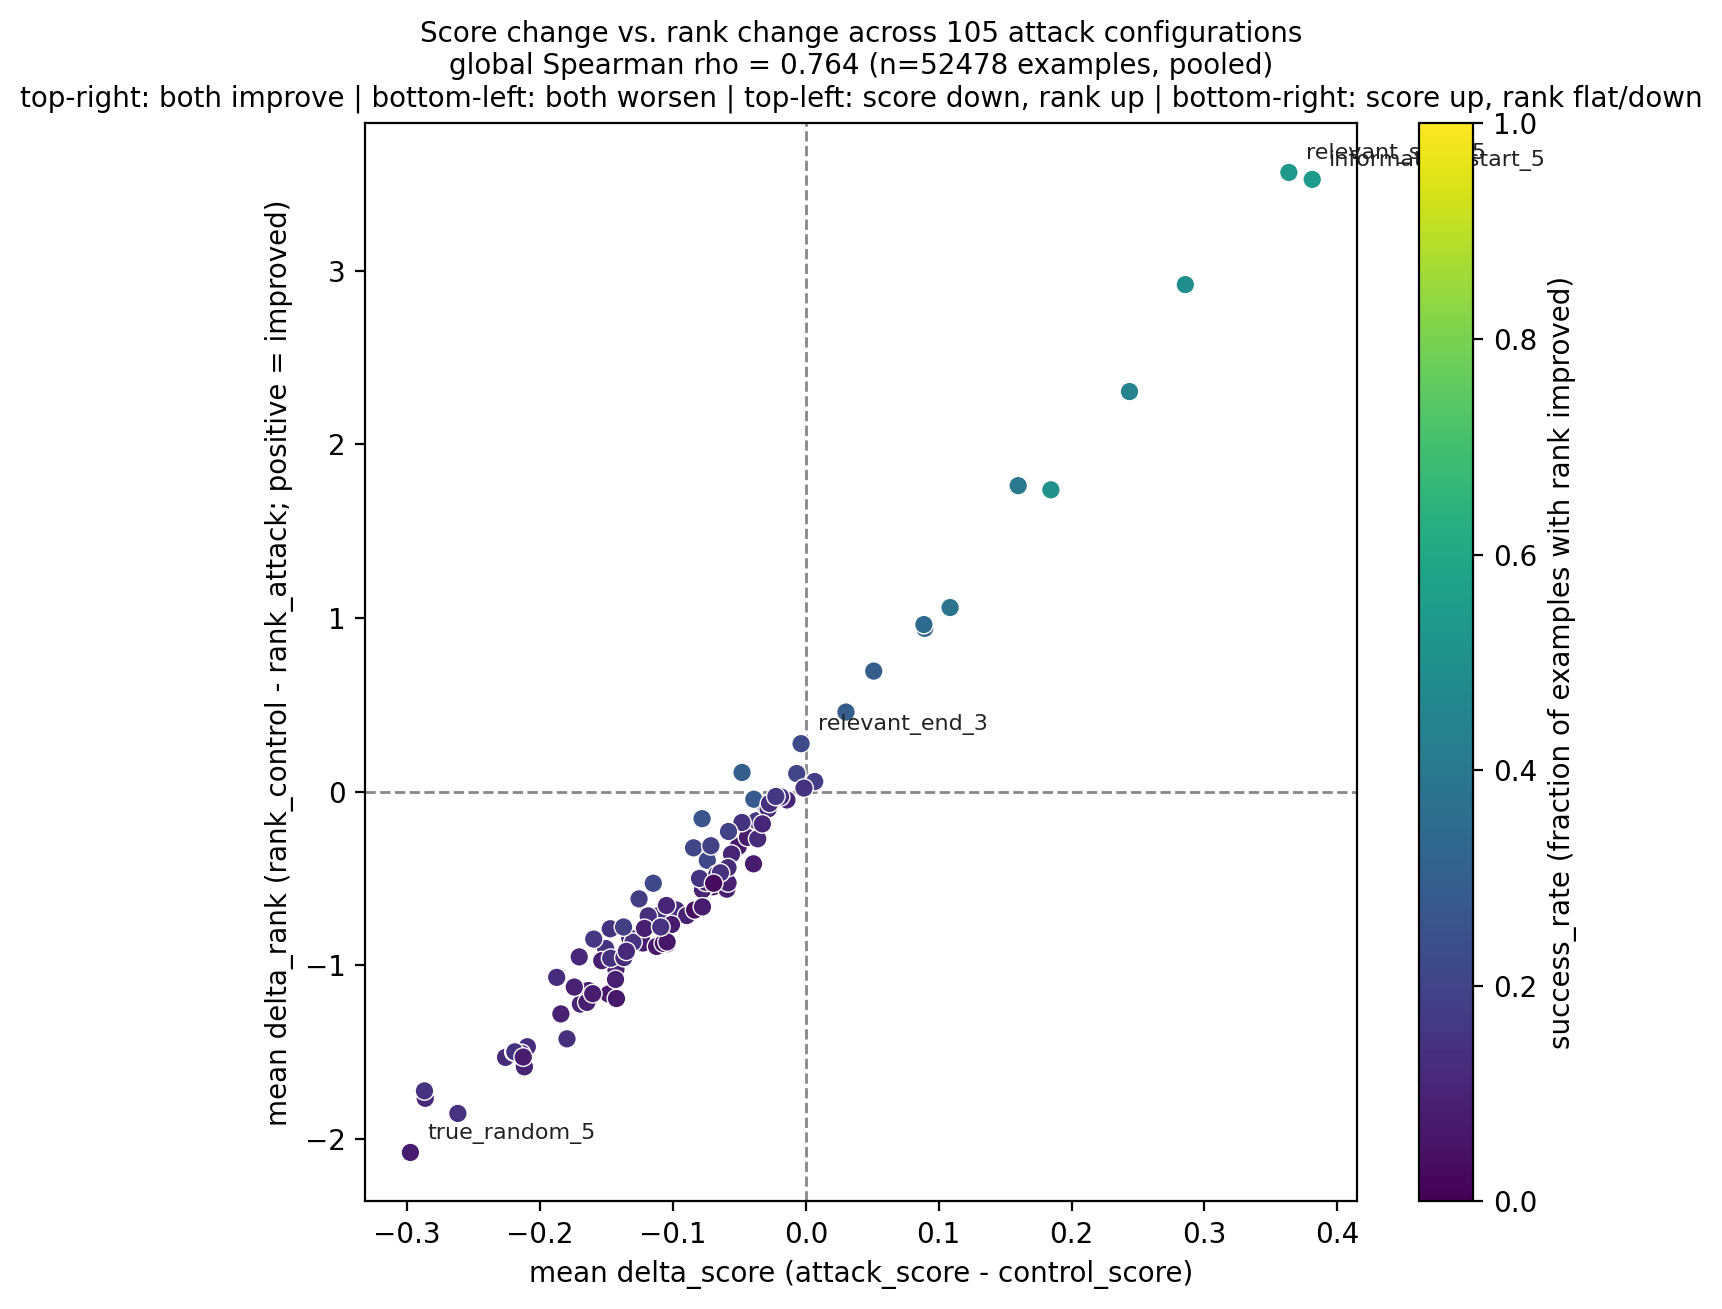
\includegraphics[width=0.85\textwidth]{outputs/plots/score_vs_rank_scatter.png}
  \caption{One point per attack configuration (105 points): mean score
  change vs.\ mean rank change, coloured by success rate. Dashed lines
  divide the plot into four quadrants (Section~\ref{sec:quadrants}).}
  \label{fig:scatter}
\end{figure}

\paragraph{Interpretation.} The per-attack scatter (Figure~\ref{fig:scatter})
is visually close to a single upward-sloping line, and the pooled,
per-example correlation ($\rho=0.764$) confirms this holds at the
individual-example level, not just in attack-level averages. \textbf{Score
change and rank change measure genuinely related phenomena}: monoT5's
raw confidence shift is a good --- though, as expected, imperfect ---
predictor of whether an attack actually improves a document's competitive
position.

\subsection{Which attacks are strongest, by both metrics}

\begin{table}[H]
\centering
\caption{Top 5 and bottom 5 attacks by \texttt{mean\_delta\_score}, with
their rank-side statistics. $n\approx500$ per row.}
\label{tab:topbottom}
\begin{tabular}{lrrrr}
\toprule
Attack & Mean $\Delta_{\score}$ & Mean $\Delta_{\rank}$ & Success rate & $\rho$ (per-attack) \\
\midrule
\texttt{information\_start\_5} & $+0.381$ & $+3.53$ & $0.544$ & $0.829$ \\
\texttt{relevant\_start\_5}    & $+0.364$ & $+3.57$ & $0.530$ & $0.827$ \\
\texttt{relevant\_start\_4}    & $+0.286$ & $+2.92$ & $0.490$ & $0.831$ \\
\texttt{information\_start\_4} & $+0.244$ & $+2.30$ & $0.444$ & $0.845$ \\
\texttt{information\_end\_5}   & $+0.184$ & $+1.74$ & $0.500$ & $0.702$ \\
\midrule
\texttt{true\_random\_5}      & $-0.298$ & $-2.08$ & $0.074$ & $0.714$ \\
\texttt{relevant\_random\_5}  & $-0.287$ & $-1.72$ & $0.146$ & $0.748$ \\
\texttt{false\_random\_5}     & $-0.286$ & $-1.77$ & $0.117$ & $0.788$ \\
\texttt{relevance\_random\_5} & $-0.262$ & $-1.85$ & $0.142$ & $0.790$ \\
\texttt{bar\_random\_5}       & $-0.226$ & $-1.53$ & $0.124$ & $0.770$ \\
\bottomrule
\end{tabular}
\end{table}

\paragraph{Interpretation.} These rankings reproduce Experiment~1's
score-only attack-strength findings almost exactly (\texttt{information\_start\_5}
and \texttt{relevant\_start\_5} as the strongest attacks, all five-repetition
\texttt{random}-position attacks among the weakest/most self-defeating) ---
an independent cross-check, since this experiment recomputed nothing about
attack strength itself and simply re-read Experiment~1's existing scores.
What is new here is that the \emph{same} ranking, by \emph{success rate}
and \emph{mean rank change}, agrees: the two strongest score-based attacks
are also the two attacks whose average target most improves its actual
competitive rank (mean rank improvement of $+3.5$ positions, more than
half the examples strictly improving rank), and the weakest/negative
score-based attacks are the ones whose targets are, on average, actively
pushed \emph{down} the ranking.

\subsection{Quadrant analysis}
\label{sec:quadrants}

\begin{table}[H]
\centering
\caption{Attack configurations by quadrant (105 total).}
\label{tab:quadrants}
\begin{tabular}{lrl}
\toprule
Quadrant & Count & Interpretation \\
\midrule
Top-right (score $\uparrow$, rank $\uparrow$)   & 12 & Both metrics agree the attack helps. \\
Bottom-left (score $\downarrow$, rank $\downarrow$) & 89 & Both metrics agree the attack hurts (or is net-neutral/negative). \\
Top-left (score $\downarrow$, rank $\uparrow$)  & 4  & Disagreement: worth inspecting individually. \\
Bottom-right (score $\uparrow$, rank$\,\not\uparrow$) & 0 & Disagreement: \textbf{empty}. \\
\bottomrule
\end{tabular}
\end{table}

\paragraph{Interpretation.} Only \textbf{4 of 105} attack configurations
land in a quadrant where the two metrics disagree in sign, and the
\emph{other} disagreement quadrant (bottom-right: score improves but rank
does not) is \textbf{completely empty} --- no attack configuration in this
grid ever raises the average score without also raising the average rank.
This is a meaningful asymmetry: when the two metrics diverge, it is only
ever in the direction of rank improving \emph{more} than score would
suggest, never the reverse. The four top-left (disagreement) attacks are
\texttt{relevance\_start\_5} ($\Delta_{\score}=-0.048$,
$\Delta_{\rank}=+0.11$), \texttt{information\_end\_2} ($-0.007$, $+0.10$),
\texttt{relevant\_end\_3} ($-0.004$, $+0.28$) and \texttt{relevance\_end\_1}
($-0.001$, $+0.02$) --- all four have a mean score change extremely close
to zero (largest magnitude $0.048$, an order of magnitude smaller than the
top attacks in Table~\ref{tab:topbottom}), so these are examples of
attacks that are \emph{roughly score-neutral on average} while still
producing a small, real net rank improvement for some examples --- not
cases of a strong, confidently-measured disagreement between the two
metrics. Notably, \texttt{relevance\_start\_5}'s \emph{per-attack} Spearman
correlation ($\rho=0.845$, the second-highest of all 105 attacks) is
actually excellent despite its negative \emph{mean}: this is an attack
whose individual examples are strongly score/rank-correlated, but whose
average happens to sit just barely on the negative side of zero, a useful
reminder that the per-attack \emph{mean} and the per-attack
\emph{correlation} answer different questions.

\subsection{Robustness check: originally-in-candidate-set vs.\ not}
\label{sec:robustness}

Because $90.2\,\%$ of examples were not originally within their query's
top-100 (Section~\ref{sec:coverage}), it is natural to ask whether the
headline correlation is being driven mainly by the (larger) out-of-set
subgroup, where a document's rank against a top-100 field it never
competed in is a somewhat more artificial counterfactual.

\begin{table}[H]
\centering
\caption{Score/rank correlation split by whether the target was originally
a top-100 BM25 candidate.}
\label{tab:robustness}
\begin{tabular}{lrrr}
\toprule
Group & $n$ & Success rate & Spearman $\rho$ \\
\midrule
Originally in top-100      & 5{,}145  & $0.240$ & $0.833$ \\
Originally NOT in top-100  & 47{,}333 & $0.146$ & $0.754$ \\
\bottomrule
\end{tabular}
\end{table}

\paragraph{Interpretation.} If anything, the correlation is
\textbf{stronger}, not weaker, for the genuinely competitive subgroup
($\rho=0.833$ vs.\ $0.754$) --- confirming the headline result is not an
artefact of the majority out-of-set subgroup and is, if anything, an
\emph{understatement} of how well the two metrics agree among documents
that were realistically competing for a ranking position. Originally-in-set
targets also see a higher success rate ($24.0\,\%$ vs.\ $14.6\,\%$) and
larger-magnitude rank swings ($|\Delta_{\rank}|=2.26$ vs.\ $1.50$ on
average) --- unsurprising, since a document already near the top of its
field has more room to visibly move within the bounded $[1,101]$ rank
scale that a deeply-buried document mostly cannot reach regardless of how
much its score changes.

% =====================================================================
\section{Overall Interpretation and Discussion}
% =====================================================================

\begin{enumerate}
  \item \textbf{This project's score-based results do not contradict
        Parry et al.'s rank-based results.} The two metrics correlate
        strongly ($\rho=0.764$ pooled, $0.53$--$0.85$ per individual
        attack) and rank essentially the same attacks as strongest/weakest.
  \item \textbf{The relationship is asymmetric in a specific, informative
        way.} Score improvements essentially always translate into rank
        improvements (the bottom-right disagreement quadrant is empty
        across the full 105-attack grid), while a small number of
        near-zero-score attacks can still produce a modest net rank
        improvement --- rank is, in this sense, a slightly more permissive
        measure of ``the attack did something'' than raw score change.
  \item \textbf{The correlation survives, and even strengthens, when
        restricted to targets that were realistically competing for a
        ranking position} (Section~\ref{sec:robustness}), addressing the
        natural concern that computing a ``rank'' for documents nowhere
        near the top-100 might be a weak or artificial signal.
  \item \textbf{Practical implication.} Future experiments in this project
        can continue reporting the (cheaper, no-candidate-set-required)
        score-based metric with reasonable confidence that it reflects real
        rank movement, while this report provides the quantitative bridge
        back to Parry et al.'s rank-based framing whenever both are needed
        side by side.
\end{enumerate}

% =====================================================================
\section{Limitations and Threats to Validity}
% =====================================================================

\begin{itemize}
  \item \textbf{Point-wise, single-document rank counterfactual.} Only the
        target document's score is swapped; the other 99 candidates always
        keep their clean scores, matching Parry et al.'s and DecoderLens's
        own protocol, but this means simultaneous multi-document attacks
        (e.g.\ several competing documents attacked at once) are not
        modelled.
  \item \textbf{Fixed candidate-set size (100).} A document's rank is
        capped at $[1,101]$; two attacks that both push a deeply-buried
        document ``closer to the top-100 but still outside it'' are
        indistinguishable by $\Delta_{\rank}$ even if their underlying
        score changes differ substantially.
  \item \textbf{Ties and rank granularity.} Rank is an integer; small,
        real score changes that do not cross another candidate's score
        produce $\Delta_{\rank}=0$, which is a legitimate ``no visible
        rank effect'' result but adds a floor of noise to any per-example
        correlation.
  \item \textbf{Single model/dataset.} Results are for monoT5-base on
        DL19's 42 queries, matching the rest of this project.
\end{itemize}

% =====================================================================
\section{Reproducibility}
% =====================================================================

From the experiment directory, with the \texttt{advseq2seq} conda
environment:

\begin{lstlisting}
python scripts/01_build_candidate_scores.py --config configs/default.yaml  # one-time
python scripts/02_compute_score_rank.py     --config configs/default.yaml  # 0 forward passes
python scripts/03_aggregate.py               --config configs/default.yaml
python scripts/04_make_plot.py                --config configs/default.yaml
# or, equivalently:
bash bash/run_all.sh configs/default.yaml
\end{lstlisting}

\noindent Total new model inference for the entire experiment is
$\sim$4{,}300 forward passes (script~01 only); scripts~02--04 are pure
CSV/dict/plotting logic. A CPU-only smoke config
(\texttt{configs/smoke.yaml}, 3 attacks, top-20 candidates) and an 8-test
\texttt{pytest} suite (import-collision regression test, candidate/target
dedup logic, metric formulas) verify the pipeline before a full run.

% =====================================================================
\section*{Appendix: Glossary of Key Quantities}
\addcontentsline{toc}{section}{Appendix: Glossary of Key Quantities}
% =====================================================================

\begin{description}[leftmargin=1.6em,style=nextline]
  \item[$\score$] $\operatorname{logit}(\texttt{true})-\operatorname{logit}(\texttt{false})$ at the first decoder step.
  \item[$\Delta_{\score}$] $\score_{\text{attack}}-\score_{\text{control}}$, read directly from Experiment~1's data.
  \item[$\rank$] 1-indexed position within a query's fixed top-100 BM25 candidate set, 1 = best.
  \item[$\Delta_{\rank}$] $\rank_{\text{control}} - \rank_{\text{attack}}$; positive = moved toward rank~1.
  \item[success] $\mathbb{1}[\Delta_{\rank}>0]$, per example.
  \item[$\rho_{\text{global}}$] Spearman correlation between $\Delta_{\score}$ and $\Delta_{\rank}$, pooled across all 52{,}478 examples --- the headline number.
  \item[Experiment 8 / DecoderLens] \texttt{monot5\_decoderlens\_rank/}, source of the candidate-set and rank-computation code (not its precomputed run outputs --- see Section~\ref{sec:coverage}).
\end{description}

\end{document}
